\documentclass[border=2pt]{standalone}
\usepackage{tikz}
\usetikzlibrary{shadings}

\begin{document}
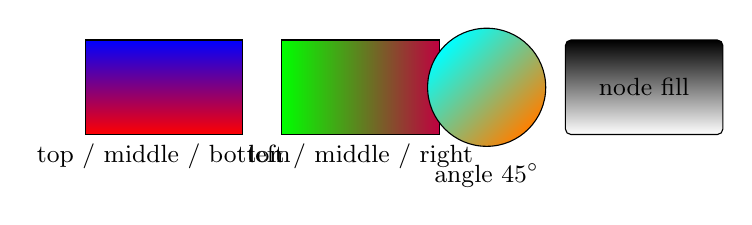
\begin{tikzpicture}[font=\small]
  \shade[draw=black, top color=blue, middle color=white, bottom color=red]
    (0,0) rectangle (2,1.2);
  \node[below] at (1,0) {top / middle / bottom};

  \shade[draw=black, left color=green, middle color=yellow, right color=purple]
    (2.5,0) rectangle (4.5,1.2);
  \node[below] at (3.5,0) {left / middle / right};

  \shade[draw=black, top color=cyan, bottom color=orange, shading angle=45]
    (5.1,0.6) circle [radius=.75];
  \node[below] at (5.1,-.25) {angle $45^\circ$};

  \node[draw, rounded corners=2pt, top color=black, middle color=gray, bottom color=white,
        minimum width=2cm, minimum height=1.2cm] at (7.1,.6) {node fill};
\end{tikzpicture}
\end{document}
